%!TEX root = ../../dissertation.tex
%%%%%%%%%%%%%%%%%%%%%%%%%%%%%%%%%%%%%%%%%%%%%%%%%%%%%%%%%%%%%%%%%%%%%%%%%%%%%%%%
\section{Recent Developments in the Mobile Network Stack}
\label{c5:sec:stack-enhancements}


Contrary to the popular scientific belief, that the Internet is unable to change and renew itself (so called Internet ``ossification'', compare, e.g., \cite{feldmann2010ossification}), protocols in the \gls{TCP}/\gls{IP} stack change all the time. Changes are more likely to occur in the end-to-end stack behavior and not in the packet format, as they are more difficult to change. New application requirements and changing network architectures always trigger adaptations in the stack in-between. 

This section briefly covers the existing protocol stacks in relation to mobile networks and streaming, new protocols and how they might influence the stack, and also discusses \gls{TCP} more closely as an example. Beneficial interactions between the stack's layers are presented in a final part.

%%%%%%%%%%%%%%%%%%%%%%%%%%%%%%%%%%%%%%%%%%%%%%%%%%%%%%%%%%%%%%%%%%%%%%%%%%%%%%%%
\subsection{Influences of the Existing Stack}
\label{c5:sec:stack-influences}

Superficially not much has changed in the Web's protocol stack. There is still \gls{IP}, \gls{TCP}, and \gls{HTTP} forming effectively the same protocol stack since 1991 with HTTP/0.9. And this seems hard to change, especially the transport layer is fixed to \gls{UDP} and \gls{TCP}, everything else will probably get rejected, altered or even dropped by one of the numerous middleboxes, such as \glspl{NAT}, or forced ``traffic optimization'' transparent proxies, all of which are especially prevalent in mobile networks \cite{sigcomm11middleboxes}. As a side note, this adds another layer of state kept in the network. A fact that was already discussed as being highly problematic and capable of inducing load in the core network in Chapter~\ref{chap:mobilenets}.

Each protocol, representing a layer in the stack, characteristically contributes to influencing data transmissions and varies in its degree of impact on the network as well as the intended goal of the transmission (e.g., streaming and watching a video).

\begin{figure}[htb]
	\centering
	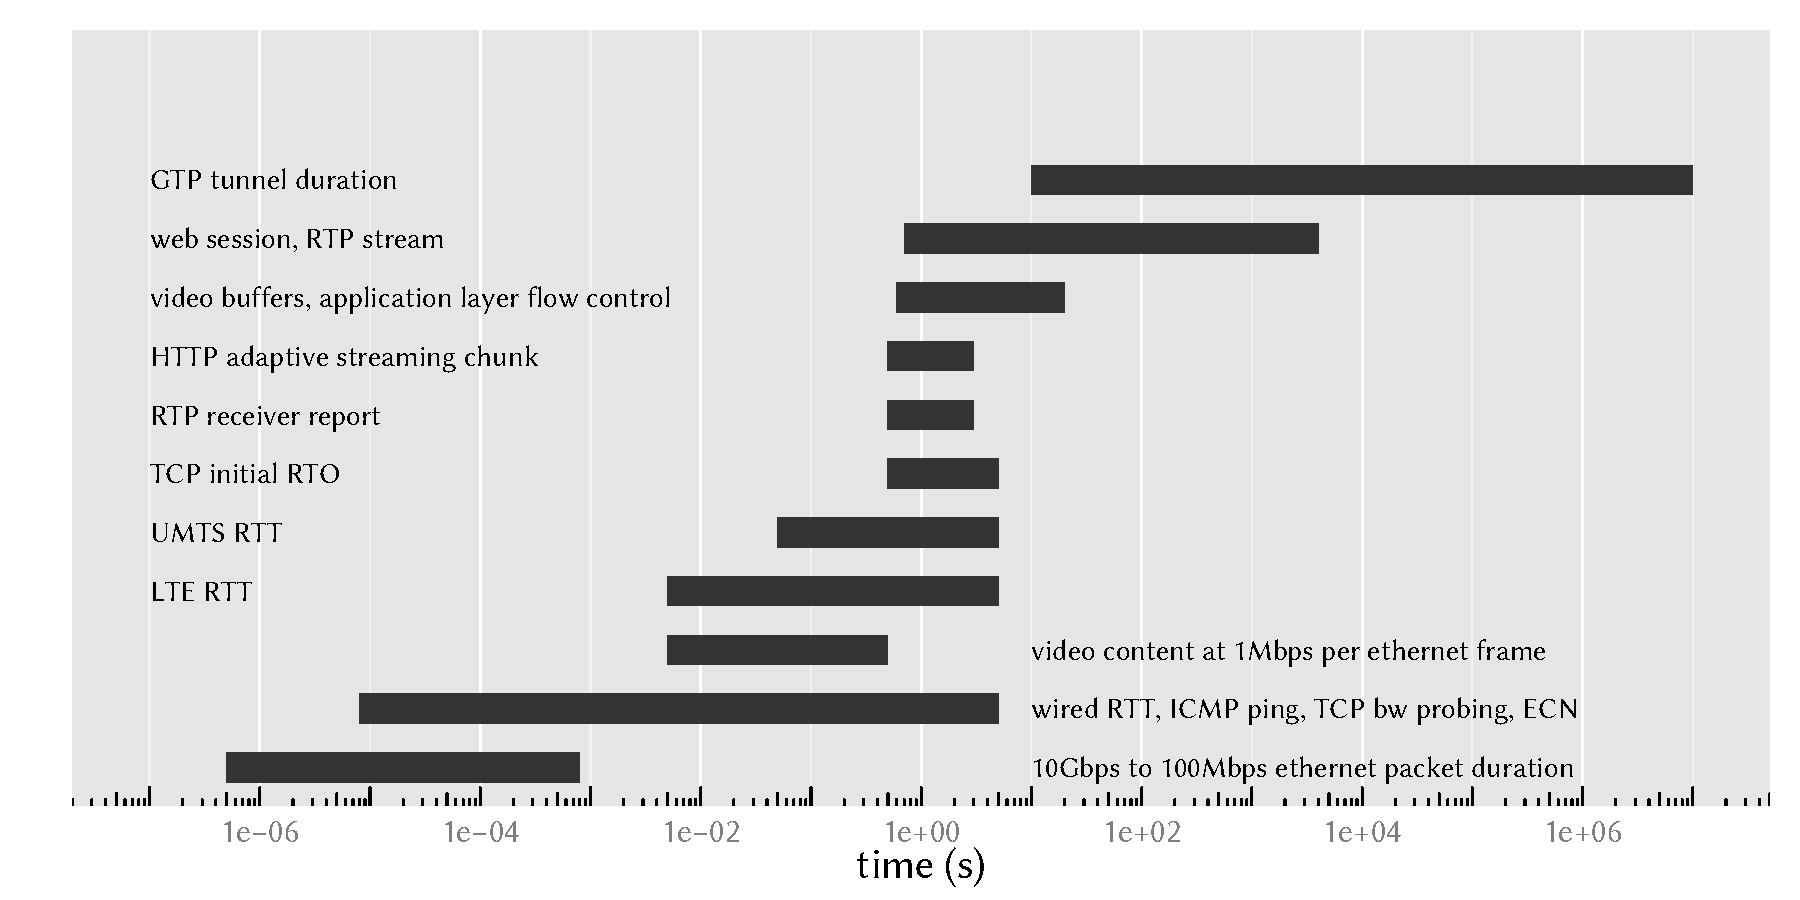
\includegraphics[width=1.0\textwidth]{images/layer-timescales.pdf}
	\caption{Approximate discernible time scales the networking stack protocols operate on in each layer.}
\label{c5:fig:timescales}
\end{figure}

Associated with each layer, and with the actual application running on top of the stack as well, are different timing constraints or time constants of control. Figure~\ref{c5:fig:timescales} overviews the approximate time scales on which activities take place, spanning a remarkable range of twelve orders of magnitude. Complexity is introduced by stacking multiple layers on top of each another, with many layers bringing along their own notion of control and feedback loops. Functionality might be duplicated across different layers, e.g., flow control in the application and on transport layer, leading to nested control loops, which might be coupled due to the timing constraints.

From the application layer end-to-end perspective the mobile network protocols seem to simply increase the depths of the protocol stack. Still, there are effects present that are specific to wireless access and mobile networks differ from the notion of an underlying wired ``dumb'' bit pipe.

First, typical effects of wireless connectivity relating to physical phenomena like fading and interference can be observed. Interruptions in the radio link are a major source of packet loss and spiking delay.
The overall delay in a mobile network is also strongly dependent on the mobile network technology used and has considerably decreased over the last few specification evolutions, even the core network. This was investigated in  \cite{laner2011dissecting3gdelay}. But even with the latest version is the \gls{RAB} and \gls{gtp} tunnel setup --- as previously described in \ref{c4:3gpparchitecture} --- sufficiently lengthy to be measurable and influence packet delay on initiating connections \cite{arlos2010packetsizedelayinfluence}.

To save radio and network resources devices usually have to quickly release their alloted slots causing additional delay for applications during connection reestablishment. Moreover, mobile networks offer many control options and parameters that can further influence any of the upper layers. Mobile devices have the tendency to be somewhat sensitive to some of these changes. For example, the authors of \cite{sigcomm11middleboxes} show the impact from protocol manipulations conducted by middleboxes. 

Comparing all these factors to wired protocols such as 802.3 Ethernet it is clear, that much more can happen in the mobile stack. Today Ethernet is a point to point protocol, transmission delay depends only on very few predictable factors, such as the distance. Wired access is typically not conducted solely through Ethernet, but with access technologies such as \gls{DSL} using \gls{PPPoE} or cable with \gls{DOCSIS}. While they also add more layers to wired access, they should be by far less influencing than the mobile stack. The latter has to additionally manage mobility and the shared wireless radio medium with protocols such as \gls{RLC} and \gls{RRC}.

A further details is the interaction between mobile network frame sizes and the \gls{IP} \gls{MTU}. Usually \gls{IP} adapts its packet size to the shortest frame size of all the link layer links in the path using \gls{PMTU} discovery as described in \cite{rfc1191}. Unfortunately, this can not work in \gls{3G} mobile networks, user packets are transparently fragmented by the radio protocols to fit into the transmission slots alloted to the device. For example, a \gls{GPRS} transmission slot has a length of only \SI{576.9}{\micro\second} carrying just \SI{114}{\bit}. And in \gls{UMTS} \SI{40}{\byte} of payload are typically carried in each \gls{RLC} frame (with optional header compression in the \gls{PDCP} layer).

% http://etutorials.org/Mobile+devices/gprs+mobile+internet/Chapter+1+Introduction+to+the+GSM+System/Radio+Interface/
% http://books.google.at/books?id=Vk9AmYz7TfoC&pg=PA184&lpg=PA184&dq=umts+pdu+size&source=bl&ots=jeO-rpM8HK&sig=NB2FAB37YcdyujYUt_kaHYwLEOE&hl=en&sa=X&ei=KjCxU6C-FKip0AXh94GQDw&redir_esc=y#v=onepage&q=umts%20pdu%20size&f=false

This fragmentation is another source of an undesired interaction between \gls{3G}'s link layer and everything above and including the network layer, potentially fragmenting packets over a long period and thereby causing delay.

In a neutral network, all packets are treated the same and should be subject to the same \gls{RTT} influencing sources.
However, delays in the delivery of data to the upper layers can occur due to certain protocol features, such as \gls{TCP} retransmissions. After being detected through timers or duplicate acknowledgments any lost packet is automatically retransmitted by the sender. Therefore, loss from the lower layers is hidden from the application layer at the cost of delay variations and probably increased overall delay. The increase in delay is especially noteworthy in any \gls{3G} cellular network with its notion of link layer \gls{ARQ} and mobility. With the latter concept, transmissions originally running through one radio tower are redirected to a new tower after a handover, even if the handover period was lengthy. These two combined can be the source of very high delay, reaching seconds to even hundreds of seconds, when moving quickly between coverage areas (e.g., in a car or train). 
This also causes bad interactions with \gls{TCP}, as these long-delayed segments are thought to be lost and subsequently retransmitted, resulting in an even further increase of delay and delay jitter.

Another undesirable influence factor is caused by each packet buffer in the transmission's path. The effect occurs if the size of the buffer is not chosen carefully and the following link is a bottleneck link. Additionally, memory is very cheap, so hardware vendors tend to plug in as much as they can and advertise it as a feature. Packets may be kept unnecessarily long in these buffers, heavily increasing packet delay and diminishing \gls{TCP}'s ability to adapt itself to its fair share with the congestion control mechanisms~\cite{jacobson1988congestion,scharf2011comparison}. These mechanisms rely on feedback from the network by inducing packet loss which does not happen in a timely manner in case of large buffers. This phenomenon is called \textit{Bufferbloat}, and can induce latency as high as several seconds~\cite{gettys2011bufferbloat,groenewegen2011detecting}. And this is in addition to the latency in mobile networks, that is already high and unreliable to begin with.

Buffers are necessary to compensate for short-term variations in the traffic load and avoid loss in these situations. A popular countermeasure are \gls{AQM} methods, that control the size of the buffer and selectively drop packets if necessary. Although, most of these are never widely used because of configuration issues. One particular algorithm stands out, that is becoming increasingly popular: CoDel~\cite{Nichols:2012:CQD:2209249.2209264, nichols2014codel}.

CoDel measures the time it takes for a packet to pass through a buffer and begins dropping packets once a certain limit has been surpassed in a predefined interval. This and other similar mechanisms that control queue delay and not its size have begun to appear and be used in several places, e.g. in the Linux Kernel.

Up to the point of the transport layer the layers are pretty well defined, with only a few select protocols to choose from, all with well known influence factors on the mobile network. The application layer has a different notion, though. Adhering to the end-to-end design principles most innovation (and therefore change) will take place at the utmost ends, i.e., the application layer. Even when only considering video streaming applications the protocol variations are countless as the overview and classification in Section~\ref{c3:background} demonstrated. 

In streaming over mobile networks the video buffer size has to be in the range of seconds to compensate for most eventualities as seen in Figure~\ref{c5:fig:timescales}. And every streaming protocol has slightly different time scales and feedback loops.

As is the case in any best-effort network no bandwidth, latency, or loss guarantees can be given. The available bandwidth might get unexpectedly smaller resulting in a quickly draining video buffer if it was chosen too small. Then again, given sufficient bandwidth stability or at least predictability, buffer sizes could also be kept at a bare minimum, thereby enabling or improving real-time interactivity. In addition to a fitting choice of the buffering and playback strategies the choice of segment length and quality levels in adaptive streaming also plays an influential role in mobile networks. Most of these factors were discussed in Chapter~\ref{chap:streaming}.

In layered network models individual functions are strictly separated and stacked on top of each other with well-defined \glspl{API} connecting them. To achieve complete separation without cross-influences, the feedback and control loops of each layer also would need to operate on completely disjoint time scales.

Looking again at Figure~\ref{c5:fig:timescales}, it can be seen that this notion is only partly supported and the loops of adjacent layers typically overlap somewhat. Protocols and implementations need to be aware of this circumstance and able to handle cross-layer influences.


%%%%%%%%%%%%%%%%%%%%%%%%%%%%%%%%%%%%%%%%%%%%%%%%%%%%%%%%%%%%%%%%%%%%%%%%%%%%%%%%
\subsection{Recent and Upcoming Protocols}

Protocol development has not stopped in recent years. On the contrary, some interesting changes are occurring especially in the application and transport layers. The following paragraph highlight some of the changes and their potential influence on mobile streaming.

Beginning at the transport layer some alternative approaches to \gls{TCP} are available, as especially the retransmission reliability has proven to be problematic in mobile networks as discussed. Typically, \gls{TCP} is used nonetheless because of two reasons: First, having congestion control is an absolute necessity to achieve an equal fair share and avoid congestive collapse and would otherwise have to be implemented in the application layer when using just \gls{UDP}. This generates additional implementation work and simultaneously reduces portability and compatibility to other congestion control variants --- the term \textit{TCP friendliness} has been used here. Second, due to many middleboxes simply dropping any unrecognized protocol --- exempting \gls{UDP} and \gls{TCP} --- the transport layer protocol often can not be changed at will and new transport protocol approaches would need to layer themselves atop \gls{UDP} incurring additional overhead.

These following three are examples of transport protocols each created with different goals in mind:

\begin{itemize}
\item \gls{DCCP}~\cite{rfc4340} extends \gls{UDP} with data flows and \gls{TCP}-compatible congestion control omitting the strict retransmission feature.

\item The \gls{LEDBAT}~\cite{rfc6817} congestion control algorithm which is implemented, amongst others, in \gls{uTP}~\cite{bt2010utp} used in file-sharing. Traffic using \gls{LEDBAT} is of high volume, high elasticity, and low priority. Data handled by this congestion control approach gets displaced by any other data if the algorithm detects an increase in the transmission buffer delay.

\item \gls{QUIC}\footnote{\url{http://lwn.net/Articles/558826/} and \url{http://www.ietf.org/proceedings/88/slides/slides-88-tsvarea-10.pdf}} is a further experimental approach aimed at reducing sources of latency spikes which would occur in \gls{TCP}, such as retransmissions or the initial handshake. Some reliability is achieved through \gls{FEC} schemes if desired. Furthermore, a novel congestion control mechanism based on packet pacing, not through a traditional congestion window, and encryption by default are implemented. However, it is not intended as a production protocol but is rather a testbed for future mechanisms and modifications to existing protocols.
\end{itemize}

In the wake of Edward Snowden's surveillance and man-in-the-middle reveals, uncovering programs such as \todo{citation needed} the \gls{IETF} announced its position on these issues in \gls{RFC}~6973~\cite{rfc6973} suggesting, that all future standardized protocols should consider surveillance issues and minimize or prevent any attempt. Ultimately, this might lead to a end-to-end \textit{crypto-by-default} Internet, with every protocol providing at least opportunistic encryption. The first signs are already visible in today's traffic mix, with many Websites only available through \acrshort{HTTPS} --- using \gls{TLS}~\cite{rfc5246} --- any more. Similarly most e-mail providers have moved to \acrshort{IMAPS} and \acrshort{SMTPS}, even using new authentication and key exchange techniques like \gls{DANE}~\cite{rfc6698} which in turn relies on \gls{DNSSEC}~\cite{rfc4033} to authenticate the validity of \gls{DNS} entries. For example, the current draft version of HTTP2 --- which will be described in more detail shortly --- mandates the presence, albeit not the usage, of \gls{TLS} capability in both client and server. And even the connectionless \gls{UDP} can be secured using \gls{DTLS}~\cite{rfc6347}.

Usually, an additional intermediate layer is added through the encryption process, adding more timing interdependencies to the other layers. However, end-to-end encryption also diminishes the influence of most middleboxes as they are not able to alter the contents of the --- now encrypted --- segment any more.


Moving on to the application layer, some interesting developments have occurred in the Web's stack and in its use of \gls{HTTP} which almost all reliable streaming methods facilitate.

The original HTTP/1.0 specification is from the year 1996 with only one update to HTTP/1.1 in 1999 thereafter. Since then, no changes have been made to the core protocol. The number of use cases facilitating \gls{HTTP} has increased significantly, bringing with them a lot of long-standing issues that were not though of initially.

The typical number of individual \gls{HTTP} requests for one Web page has steadily increased, reaching today over \numprint{100} objects.\footnote{\url{http://www.websiteoptimization.com/speed/tweak/average-web-page/} and \url{http://www.httparchive.org/trends.php?s=All&minlabel=Nov+15+2010&maxlabel=Jul+1+2014} and \url{https://developers.google.com/speed/articles/web-metrics}} \gls{HTTP} deals with this through persistent connections and pipelining to avoid unnecessary connection establishment and request delays. Pipelining is however disabled in almost every client implementation as it suffers from head-of-line blocking. To circumvent this problem and increase retrieval speed, browsers have begun to open many parallel \gls{TCP} connections per site, invoking significant overhead and general fairness issues due to the large number of \gls{TCP} connections displacing other traffic.

Moreover, the Web's structure has changed in such a way, that it is now common to push data to the clients to increase a Web page's interactivity. However, \gls{HTTP} is a simple client-initiated request-response protocol and pushing can only be emulated using techniques such as \textit{long polling} which imposes several restrictions and state overhead. Both these issues also affect reliable streaming with \gls{HTTP} to a certain degree. Streaming can benefit from a reduction of request latency as well as servers pushing adequate video segments at the correct time without the need for further requests.

To combat the situation and increase the protocol's interactivity along with it, several approaches are being developed. The first, WebSocket~\cite{rfc6455}, is a transport protocol on top of \gls{TCP} (or \gls{TLS}) that can be established through a regular \gls{HTTP} connection. It enables full-duplex communication between the two communication nodes. An additional \gls{W3C} \gls{API}~\cite{w3c2011websockets} enables simple usage in browsers with higher interactivity than plain \gls{HTTP}. It is also used to stream content to a browser.

The \acrshort{WebRTC} protocol suite\footnote{\url{http://www.webrtc.org/}}~\cite{webrtcdraft} even goes a step further and provides a complete stack for multimedia communication. It is intended to be used --- through the provided \gls{API} --- for direct browser-to-browser communication initiated by a central server-side Web page.

Both these techniques aim to enhance or sidestep \gls{HTTP}. But it is also desirable to improve the protocol itself for the aforementioned reasons. Therefore, in 2010 Google implemented a new experimental application protocol called SPDY as an alternative to \gls{HTTP} in its browser Chrome accompanied by a draft specification~\cite{google2011SPDYdef, google2010SPDYwp}. Every major browser and most Web servers support SPDY, many Cloud and \gls{CDN} providers have it enabled.

SPDY uses the same port as \acrshort{HTTPS} (443) and mandates the use of \gls{TLS} as it also serves to negotiate the choice between \gls{HTTP} and SPDY. Compared to \gls{HTTP} pipelining, SPDY provides full-duplex time-division multiplexing. After an initial request of a Web page, the server can anticipate any follow-up requests, push objects on additional streams with assigned priorities and therefore avoid additional request round trips.

All of the SPDY changes are aimed at reducing the number of established \gls{TCP} connections for a Web site retrieval, ideally down to one, and reduce the overall latency of the object transmissions. Evaluations in \cite{google2010SPDYwp} suggest an average Web page load time reduction of \SI{29}{\percent}. The gains for networks with high latency, e.g., mobile networks, the gain could be even higher as several round trips are avoided.

Some of the benefits are also applicable to reliable streaming, with video segments being able to be pushed from the server. Conjoined with \gls{SVC}, SPDY could multiplex the different video layers in one connection, with the highest priority assigned to the base layer.

The SPDY draft was later picked up by the \gls{IETF} Httpbis working group as an initial basis basis for the \gls{HTTP} 2.0 specification~\cite{http20draft} currently being finalized as of mid 2014. It follows the SPDY specs rather closely, with the only major difference being the use of \gls{TLS}. Its usage is not mandated anymore, merely its presence and, if used, the application of strong and ephemeral cipher suites.



%%%%%%%%%%%%%%%%%%%%%%%%%%%%%%%%%%%%%%%%%%%%%%%%%%%%%%%%%%%%%%%%%%%%%%%%%%%%%%%%
\subsection{Additional TCP Changes}

In addition to the previously described new transport protocols under development aiming to replace and surpass \gls{TCP}, \gls{TCP} itself is not as static as it may seem. While the basic wire frame and data interchange format has already been defined in 1981 in RFC~793~\cite{rfc793}, much of the specific behavior is free to be experimented with by further specifications and implementations. The most prominent example is the congestion control mechanism where every operating system takes hugely different approaches.


\begin{table}[htbp]
	\begin{tabu}{X[1.4]XX[0.4]X[0.7]}
	\toprule
	\textbf{Change} & \textbf{Related Work} & \textbf{Kernel} & \textbf{Date} \\
	\midrule
	BIC as default congestion avoidance algorithm (from Reno) & & 2.6.8 & August 2004 \\
	CUBIC as default congestion avoidance algorithm & \cite{ha2008cubic} & 2.6.19 & November 2006 \\
	New TCP Slow Start: HyStart & \cite{Ha20112092} & 2.6.29 & March 2009 \\
	Multipath TCP & RFC6824 & external & 2011 \\
	TCP User Timeout & RFC5482~\cite{rfc5482} & 2.6.37 & January 2011 \\
	Initial Receive Window \SI{10}{MSS} & \cite{rfc6928} & 2.6.38 & March 2011 \\
	Initial Congestion Window \SI{10}{MSS} & RFC6928~\cite{rfc6928} & 2.6.39 & May 2011 \\
	\SI{1}{\second} initial RTO (from \SI{3}{\second}) & RFC6298 & 3.1 & October 2011 \\
	Changes to sstresh and CWND bevahior & RFC5681~\cite{rfc5681} & 3.1 & October 2011 \\ % details: https://git.kernel.org/cgit/linux/kernel/git/torvalds/linux.git/commit/?id=9ad7c049f0f79c418e293b1b68cf10d68f54fcdb
	TCP Proportional Rate Reduction & RFC6937~\cite{rfc6937} & 3.2 & January 2012 \\
	Byte queue limits and TCP buffer limits &  & 3.3 & March 2012 \\ % https://lwn.net/Articles/454390/
	CoDel AQM & \cite{nichols2014codel} & 3.5 & July 2012 \\
	TCP Early Retransmit & RFC5827~\cite{rfc5827} & 3.5 & July 2012 \\
	TCP small queues & & 3.6 & September 2012 \\ %http://lwn.net/Articles/507065/
	TCP Fast Open (client side) & \cite{cheng2014tcptfo} & 3.6 & September 2012 \\
	TCP Fast Open (server side) & & 3.7 & December 2012 \\
	TCP tail loss probe & & 3.10 & June 2013 \\ % http://tools.ietf.org/html/draft-dukkipati-tcpm-tcp-loss-probe-01
	TCP Forward RTO-Recovery & RFC5682~\cite{rfc5682} & 3.10 & June 2013 \\
	Low latency network polling & & 3.11 & September 2013 \\ %http://lwn.net/Articles/551284/ and http://www.linuxplumbersconf.org/2012/wp-content/uploads/2012/09/2012-lpc-Low-Latency-Sockets-slides-brandeburg.pdf
	Improved RTO calculation and handling of reordering & & 3.12 & November 2013 \\ % https://git.kernel.org/cgit/linux/kernel/git/torvalds/linux.git/commit/?id=0f7cc9a3c2bd89b15720dbf358e9b9e62af27126 and https://git.kernel.org/cgit/linux/kernel/git/torvalds/linux.git/commit/?id=ed08495c31bb991de636d2488abaa50b39f2ff4a
	TCP Fast Open enabled by default & & 3.13 & January 2014 \\
	TCP auto corking & & 3.14 & March 2014 \\ % https://git.kernel.org/cgit/linux/kernel/git/torvalds/linux.git/commit/?id=f54b311142a92ea2e42598e347b84e1655caf8e3
	PIE AQM & & 3.14 & March 2014 \\ % http://tools.ietf.org/html/draft-pan-aqm-pie-01 and https://git.kernel.org/cgit/linux/kernel/git/torvalds/linux.git/commit/?id=d4b36210c2e6ecef0ce52fb6c18c51144f5c2d88
	TCP Fast Open over IPv6 & & 3.16 & 2014 \\
	LISP & RFC6830~\cite{rfc6830} & 3.16 & 2014 \\
	\bottomrule
	\end{tabu}
	\caption{Assorted list of some select network stack changes in the Linux kernel, that alter \gls{TCP}'s transmission bevahior.}
\label{c5:tab:linux-stack-changes}
\end{table}


Every one of these changes can have unforeseen repercussions or great benefits for the application layer. The following paragraphs investigate some of the changes in the last few years and their implications.  Instead of implicitly exploring specific mechanism choices of closed source \glspl{os} and tracking their changes over the years, which would be extremely difficult, the \gls{TCP} implementation in the Linux kernel is taken as an example. The changes can be easily tracked by crawling through the patch sets and their commit logs of every kernel version. Sites like \url{http://kernelnewbies.org/} and \url{http://lwn.net/} simplify this process even more. Table~\ref{c5:tab:linux-stack-changes} depicts such an attempt to track the major changes affecting \gls{TCP} in the kernel.


Most of the changes plainly aim at reducing the number of required round trip times and increase the overall throughput while still maintaining fairness. This includes both small and larger changes, some of the more recent are:

\begin{itemize}
	\item The \gls{TCP} congestion window defines the maximum amount of data that can be transmit without having received any acknowledgments for the data. It is the central knob for all congestion control mechanisms.
	The initial window size was increased multiple times in the past --- from initially one segment, to three, and now to ten segments~\cite{rfc6928} ---  with the intent to accommodate for the increase in transmission bandwidth and higher expected traffic volume. With a ten segment window small \gls{HTTP} objects can be transferred without any ACK round trips reducing the average Web page load time.

	\item Another \gls{TCP} round trip can be saved by using the initial handshake itself for data transmission. \gls{TCP} Fast Open~\cite{cheng2014tcptfo} implements this and is again thought to reduce Web page load times.

	\item While the retransmission timeout is calculated through \gls{RTT} measurements, it is initially set to \SI{3}{\second}. This could add a high amount of delay if packets are lost during the handshake at the beginning of a connection. Implementations following RFC~\cite{rfc6298} set the default value to \SI{1}{\second} which may benefit especially mobile networks.

	\item The classic congestion avoidance algorithms do not work very well with networks with a large \gls{BDP} as the congestion window scaling entirely depends on the \gls{RTT}. Newer approaches reduce this dependence while also departing from the traditional linear growth congestion avoidance phase. Some of the congestion avoidance in use in today's \glspl{os} are 
		\begin{itemize}
			\item Reno~\cite{rfc5681}
			\item New Reno~\cite{rfc6582}
			\item Vegas~\cite{Brakmo:1994:TVN:190809.190317}
			\item Compound~\cite{song2006compound} (as an option in recent Windows versions)
			\item CUBIC~\cite{ha2008cubic} (default in Linux)
		\end{itemize}
\end{itemize}


All of these changes should serve to demonstrate the flux \gls{TCP} is in. It is constantly being adapted to current network and application needs. However, no adaptation or assumption as to specific applications are made on the transport layer. These kind of modifications can only be made on an end-to-end basis, i.e., at the application layer (cf. also the arguments in \cite{saltzer1984end2end}). All lower layers must be application-neutral as they could harm other application layer protocols.

This is contrary to the popular scientific claim that the Internet is ``ossified'' and cannot accommodate any new applications any more (confer for example in \cite{turner2005diversifying}). Rather, \gls{IP} and \gls{TCP} serve as the undiscriminating common carrier of every type of data at the bottleneck of the Internet's protocol hourglass model.


%\todo{add some concluding remarks on the adaptivity of TCP and the so-called hourglass model/ossified network that does not permit any changes at the hourglass's bottleneck (IP and TCP); mention again the correlations between the layers to lead over to the cross-layer section}

%Multipath TCP MPTCP~\cite{rfc6824}!
%Slow Start~\cite{rfc5681}
% HyStart~\cite{Ha20112092}






%%%%%%%%%%%%%%%%%%%%%%%%%%%%%%%%%%%%%%%%%%%%%%%%%%%%%%%%%%%%%%%%%%%%%%%%%%%%%%%%
%!TEX root = ../../dissertation.tex
%%%%%%%%%%%%%%%%%%%%%%%%%%%%%%%%%%%%%%%%%%%%%%%%%%%%%%%%%%%%%%%%%%%%%%%%%%%%%%%%
\section{Cross-Layer Information Exchange}
\label{c5:sec:crosslayerhinting}

The Internet has its historic roots deep in wired networks with a slim and well-defined network stack represented by the \gls{ISO}/\gls{OSI} or \gls{TCP}/gls{IP} model. These layers are isolated against each other. Only predefined information exchange points, or \gls{osiSAP}, at the layer borders allow for vertical communication. A typical wired \gls{TCP}/\gls{IP} Internet environment rests atop of either an Ethernet or other access technologies, e.g., \acrshort{DSL}, \acrshort{DOCSIS} or \acrshort{PON}, at the physical and link layers.

Application layer protocols often implicitly rely on the presence and characteristics of specific lower layer protocols. Though, through the layer isolation no application can precisely know or even control the current state of the lower layers. Nonetheless, they usually make assumptions on the composition and behavior of the lower layers and plan their work accordingly. 

But the access technology diversity has strongly increased through the advent of wireless technologies, and past fixed access behavioral patterns may not be applicable any more today. The protocols used for the radio transmissions behave very differently when compared to plain Ethernet and higher layers may make false assumptions. Examples for this were given in the in the discussion of the stack's influences in Section~\ref{c5:sec:stack-influences}.

It would be very desirable for transport and application layer mechanisms to be able to better understand these layers and cope with these effects. The term \textit{cross-layer interactions} or \textit{cross layer information exchange} subsumes these approaches. Specific information from one layer is made available to other interested neighboring or more distant layers. Using cross-layer techniques many of the previously introduced negative layer influences can be diminished or neutralized altogether.

The next sections describe related mechanisms in the literature, classifications and then proceed to describe a new cross-layer approach that facilitates cross-layer information to the benefit of mobile streaming. The cross-layer work presented here is rather meant as an initial proposal to be integrated into future streaming players and their playback and transmission strategies.


%%%%%%%%%%%%%%%%%%%%%%%%%%%%%%%%%%%%%%%%%%%%%%%%%%%%%%%%%%%%%%%%%%%%%%%%%%%%%%%%
\subsection{Related Cross-Layer Approaches and Classifications}

The idea of exchanging information between layers is not a particularly new one. Some specific ideas have been implemented a long time ago. The authors of \cite{Raisinghani2004720} list a number of scenarios in which cross-layer information could be used and also talk about the type of information to be shared between layers. One of the oldest and most well known cross-layer approaches is probably \gls{ECN}~\cite{rfc3168}. Here, the \gls{IP} layer of intermediate hops can signal the end nodes' \gls{TCP} layer that congestion is occurring and \gls{TCP} does not need to wait for implicit congestion signals, e.g., duplicate acknowledgments or timeouts. However, \gls{ECN} is disabled in almost every implementation as it lead to numerous problems and triggered bugs\footnote{\url{http://lkml.iu.edu//hypermail/linux/kernel/0009.1/0329.html}}. This is a risk that many cross-layer attempts may face.

A significant amount of publications is dealing with cross-layer information in wireless and mobile protocol stacks. A number of architectures have been proposed, e.g., \cite{raisinghani2004eclair, 1580937}, \cite{wang2003multi}, \cite{1200522}, and \cite{krishna2007cross}, but no actual solution seems to have been implemented in any of these.

While cross-layer typically implies a solely \textbf{vertical} --- between network layers --- exchange flow there can also be \textbf{horizontal} --- between network nodes --- components present. \gls{DLEP}~\cite{ietf2013dlepdraft} is such an example of a \textbf{diagonal} flow, providing information of a lower layer of one entity to a higher layer at another node. The \gls{DLEP}~\cite{ietf2013dlepdraft,6379143} protocol provides information available only to the (external) wireless modem or other interfaces to the routing entity of a node upon which it can act. Link characteristics such as bandwidth, latency, connection status, or information regarding neighbors can be requested.

Though, horizontal information flow in cross-layer approaches is more than often an indication of \textbf{centralization} (also called \textbf{network-assisted} or \textbf{managed}) as apposed to purely vertical \textbf{distributed} approaches. Concerning this network-assisted cross-layer exchange there are a number of approaches that aim to integrate layer cooperation into the design of new mobile network infrastructures, including \cite{zarai2010seamless} and \cite{Piamrat20111066}. Generally, information is retrieved from the clients and collected at a central manager to be used in any policy decision like mobility and radio resource management.

Going back to purely distributed approaches, in \cite{hummel2010mobilitaet} the concept of mobility awareness is discussed. The goal is to predict motion and mobility based on available information and adapt the individual network layers to react accordingly. One of the easiest to implement uses of cross-layer information is the selection of the active network interface. Current mobile devices have a wide range of network interfaces available, all with specific characteristics. The management architecture proposed in  \cite{Bonnin:2009:AMM:1503496.1503498} switches the currently used interface based on pre-configured profiles. Information from multiple layers is used to support the decision-making process.

To optimize unreliable video streaming in a WiFi network, the authors of \cite{1580941} create a control loop between the video encoder and the 802.11 \gls{MAC} layer to conduct WiFi rate control fitted to the output of the encoder. This is an example of a tight cross-layer control loop for one particular application. The link layer rate control will very likely have adverse affects on other applications using this node.

The notion of cross-layer can also be applied to non-traditional network stacks. For example, the authors of \cite{4656786} present a cross-layer model for satellite communication stacks. They additionally distinguish between two general flavors of cross-layer architectures, one with \textbf{direct} and the other with \textbf{indirect} communication. Direct exchange implements new vertical interfaces in the layers and exchanges information directly between them. The indirect alternative uses an external information broker that handles all communication in parallel to the existing layers. Similar cross-layer information can be offered to peer-to-peer overlay networks, as was for example researched in the SmoothIT project\footnote{\url{http://www.smoothit.org}}, where routing and topology information was collected and made available to interested peers~\cite{oechsner2009pushing} in order to keep traffic local and avoid using \acrshort{ISP} interdomain links.


%%%%%%%%%%%%%%%%%%%%%%%%%%%%%%%%%%%%%%%%%%%%%%%%%%%%%%%%%%%%%%%%%%%%%%%%%%%%%%%%
\subsection{Cross-Layer Model and Implications}

With these past approaches and classifications at hand, a cross-layer model suitable for video streaming in mobile networks can now be defined and the information to be exchanged specified.

\begin{figure}[htb]
	\centering
	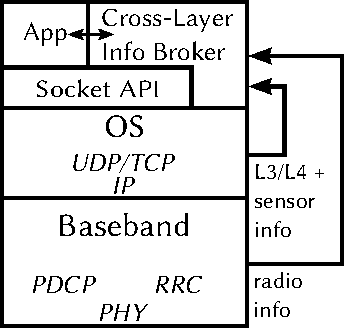
\includegraphics[width=0.3\textwidth]{images/cross-layer-model.pdf}
	\caption{Model and architecture of the proposed cross-layer information exchange.}
\label{c5:fig:crosslayer-model}
\end{figure}

Figure~\ref{c5:fig:crosslayer-model} illustrates the concept with the example of a mobile device. In a fully isolated model, no information would be passed from the baseband to the \gls{os} and the applications. The cross-layer model permits certain information to pass from one layer to another. Here, a software broker is responsible to collect information from several sources and layers and make it available to any interested application in a concise manner. 

This is an indirect cross-layer approach bypassing the intermediate layers completely and leaving them mostly unmodified. Also, information is always collected and used on the same device, making it purely vertical and distributed. Sharing this kind of information between different hosts would be accompanied by certain privacy and security implications. Most of the data is very sensitive and also be used with malicious intent if it is being leaked by a cross-layer broker.

This architecture is intended to pass data from the physical and link layer directly up to the application. Especially information specific to \gls{3G} mobile networks could be potentially interesting and used in benefit for applications and the user experience.This could include:

\begin{itemize}
	\item Information on the occurrence of a horizontal handover between cells.

	\item Information on neighboring cells and predictions when a handover is most probable to occur.

	\item Information on the prediction of the occurrence of a vertical handover and thereby changes in the active network stack, e.g., to the WiFi layers.

	\item Information on the current signal strength, bit error rate, and throughput.

	\item Detailed mobility information, including current location and travel speed in relation to base station positioning and availability.
\end{itemize}

Today, most of this information is only available inside the link layer or even just known to the mobile network's control plane. The impact of a lack of this knowledge can be significant for applications. For example, traffic scheduled during a handover period can be subject to especially high latency and loss due to the lengthy control plane interactions and traffic rerouting processes in a mobile network. If a cross-layer exchange would be provided and the application is made aware when an handover is supposed to occur, traffic could be scheduled around the event. 

Generally speaking, the goal of the cross-layer approach would be to find meaningful reactions for every type of state the lower layers report through the broker. The pool of recipients is also not necessarily limited solely to the application layer. Especially the transport layer could be interested into explicit connectivity information and be modified to react accordingly. In addition to information flow, a path for control flow could also be envisioned. Herein, applications could directly influence the decision making and policies of the lower layers and adapt them to their personal needs.

All in all, the cross-layer data needs as well as the recipient's reactions need to be well defined and thoroughly tested to avoid any conflicts and layer separation issues. The impact of a simple unidirectional information flow on the layering mechanisms is suggested to be rather low. Only explicit and specific information is revealed keeping most of the isolation intact. However, a bidirectional control flow could soften up the isolation and have adverse side-effects through conflicting interests of participating applications.

Either way, when implementing any kind of cross-layer exchange, one always has to keep a close look on the resulting consequences. One side effect can be the creation of an unintentional feedback loop between the control mechanisms of protocols of different layers. Moreover, breaches in the isolation could leak network state that could be exploited by malicious parties in any number of unforeseeable ways. Therefore, handling these plays an important role in cross-layer research. In \cite{1404568} the authors present and discuss some of these issues.


%%%%%%%%%%%%%%%%%%%%%%%%%%%%%%%%%%%%%%%%%%%%%%%%%%%%%%%%%%%%%%%%%%%%%%%%%%%%%%%%
\subsection{Utilizing Cross-Layer Information for Adaptive Reliable Streaming in Mobile Networks}

Looking at the model it can be an obvious fit for adaptive reliable streaming. As introduced in Section~\ref{c3:sec:background}, adaptive streaming usually facilitates a segment-based pull approach on top of \gls{HTTP}. A local video buffer is maintained and attempted to be kept between predefined thresholds. The goal is to never run out of buffered video while still providing the best possible quality, which could be difficult to achieve in a highly variable mobile network.

Cross-layer information can be fed into the adaptivity model of the streaming player to better decide the exact schedule and quality level of segment transmissions. Adaptive reliable streaming can be especially suited to receive cross-layer data for several reasons: First, all requests are client-initiated, so available information can be immediately taken into account and does not need to be transfered elsewhere. Second, adaptive streaming consists of small and independent video segments, which allows to quickly react on upcoming events.

\begin{figure}[htb]
	\centering
	\begin{subfigure}[b]{0.80\textwidth}
		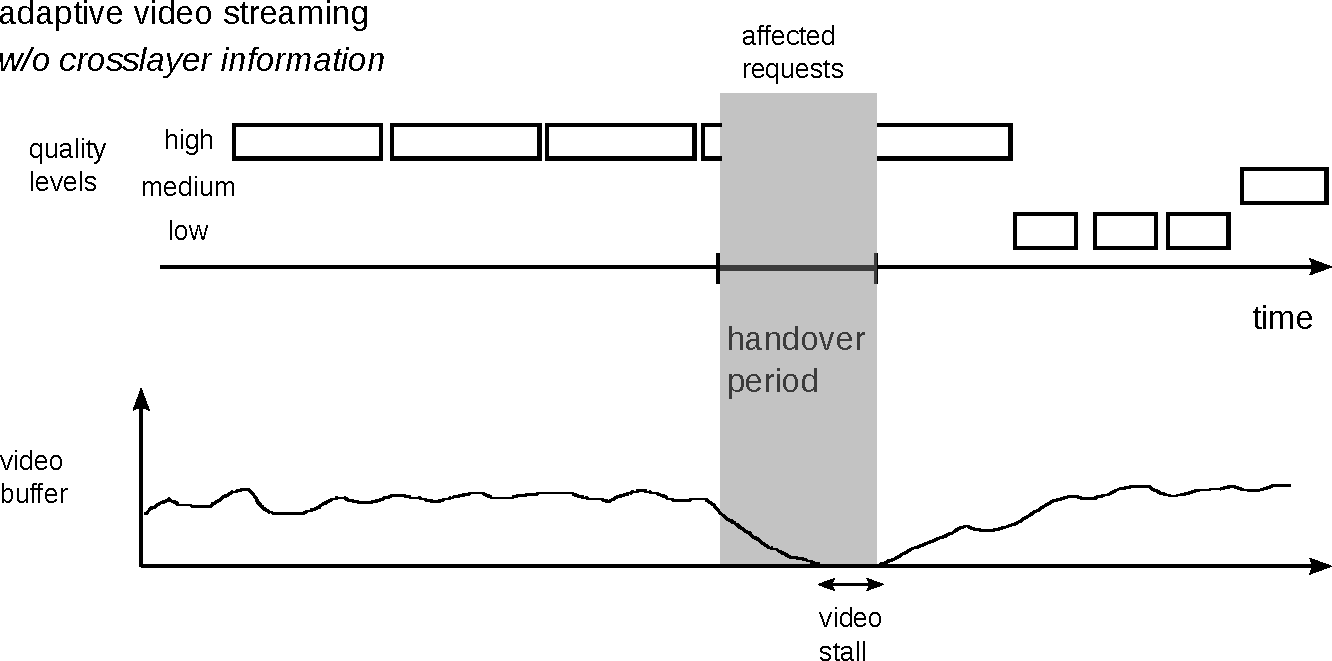
\includegraphics[width=\textwidth]{images/adaptive-streaming-no-cl.pdf}
		\caption{Stalling occurs without handover hinting.}
		\label{c5:fig:streaming-hinting-no-cl}
	\end{subfigure}%

	\begin{subfigure}[b]{0.80\textwidth}
		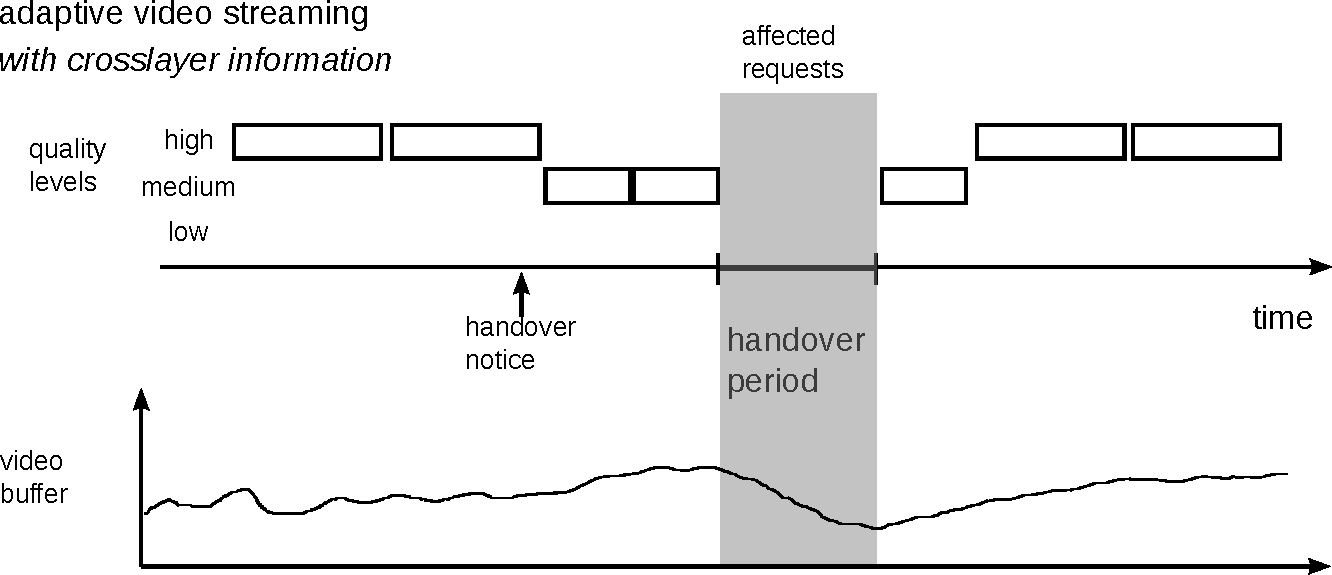
\includegraphics[width=\textwidth]{images/adaptive-streaming-cl.pdf}
		\caption{Stalling can be prevented by hinting and proactively filling the playback buffer.}
		\label{c5:fig:streaming-hinting-cl}
	\end{subfigure}%
	\caption{Adaptive video streaming scenario with and without handover prediction and cross-layer hinting.}
\label{c5:fig:streaming-hinting}
\end{figure}

One of the easiest events to improve upon is the timely knowledge (or prediction) of upcoming handover procedures, horizontal as well as vertical handovers. Consider the scenario given in Figure~\ref{c5:fig:streaming-hinting-no-cl}. The streaming player consistently retrieves video segments at the highest quality, maintaining a moderate buffer size but oblivious to the upcoming handover. This handover interrupts any transmission for a certain time, during which the buffer is fully drained and the video playback begins to stall. Only after this phase ended, the remaining portion of the segment can be received. But the buffered amount is now still below the safety margin and the player is forced to request several segments in the lowest quality to quickly refill the buffer. Only after that, the player's state normalizes and normal quality playback is restored. In summary, one unexpected service interruption causes one complete stall and a long period of reduced quality in this exemplary scenario. This effect can also be easily observed in the mobile reliable streaming simulation scenario described in Section~\ref{c6:sec:mobilitystreamingsim}.

Figure~\ref{c5:fig:streaming-hinting-cl} shows the same scenario but with cross-layer hinting present. As soon as the notice of a predicted upcoming handover is received, the streaming player can react and switch to segments with medium quality to increase the buffer size before the event. After the handover has completed one more medium segment is transmitted to get the buffer level back to normal before returning to full quality. Both the video stalling period and the drop to the lowest quality could be avoided here. The general goal in the streaming process is to both stop the buffer from ever completely emptying and also maintaining the highest possible video quality. To achieve this, early knowledge of future network conditions is highly desirable for the streaming controller to correctly adjust the segment retrieval rate and quality.

The end-to-end concept can be applied to cross-layer architectures as well. While cross-layer information can still be made available to intermediate layers, the achievable effects might either not be as large as in the highest layer or more complicated to attain. For example, it requires much more effort to correctly adjust \gls{TCP} retransmissions and congestion control to accommodate the cross-layer broker without side-effects to other applications. Nonetheless, benefits can still be attained at the transport layer to some degree if the adjustments are being kept application-neutral. This can be especially helpful for applications that have not yet been adapted to handle cross-layer information.


%%%%%%%%%%%%%%%%%%%%%%%%%%%%%%%%%%%%%%%%%%%%%%%%%%%%%%%%%%%%%%%%%%%%%%%%%%%%%%%%
\subsection{Benefits for Other Applications}

Besides this work's central motifs of reliable streaming, other applications could benefit as well. First, cross-layer information could be utilized to directly improve the user interface and experience. Any information of upcoming service interruptions or other adverse conditions are simply displayed to the user. This is specifically helpful for interactive communication --- as in video calls or \gls{VoIP}. An unsuspecting user might be more startled at a sudden loss of reception than the one that was informed beforehand. The communication partner can additionally also be informed. While user hinting and notifications does generally not actually improve the actual \gls{QoS} of the application it can still positively improve the perceived quality or \gls{QoE}. But detailed user studies would need to verify this further.

Generally, any application that can locally exert control over its traffic and does not have to rely on server-side control will benefit the most. Also, the traffic should be ideally composed of smaller objects available in multiple versions and free to be reordered. A good candidate would be Web browsers with their stateless \gls{HTTP} requests of a Web site, which is comprised of many small objects that can be, to a certain degree, requested in any order. Those objects could be requested in such an order to better accommodate network events announced by the lower layers. On the other hand, \gls{rtp}-style streaming traffic might not be able to beneficially utilize cross-layer information as just a stream of continuous data is pushed to onto the client.

Directly involving the user itself are a further category of cross-layer interactions that are only available if there is a downward control flow through the broker to the radio layer protocols. This would require the additional presence of a user-space policy manager. The manager would offer the user a series of preferences and a configuration interface for a rule-based cross-layer control engine. With this the user could create complex compound policies such as: ``Do not handover to a stationary WiFi from \gls{3G} when moving faster than \SI{50}{\kilo\meter\per\hour}, switch only to in-vehicle WiFi if available.'' or ``Avoid any vertical handover, which would interrupt my service for a long time, while a \acrshort{VoIP} call is running.''


%%%%%%%%%%%%%%%%%%%%%%%%%%%%%%%%%%%%%%%%%%%%%%%%%%%%%%%%%%%%%%%%%%%%%%%%%%%%%%%%
\subsection{Implementation Outlook and Approaches}

As the model displayed, the target applications should not be directly (or indirectly through the inclusion of a third-party software library) responsible to retrieve cross-layer information. Instead, the broker was suggested as the means to implement cross-layer exchange in an actual software environment. This daemon --- located in the user space --- collects information from the lower layer network protocols which usually reside entirely in kernel space. The kernel typically exposes only some data publicly with a stable \gls{API} and \gls{ABI}. Other data can often be derived from internal data structures which usually change with every version. The task of adapting to this changes and collecting concise data is handled by the daemon. Only the actual reactions to these information points must be implemented in the application itself.

The daemon provides all information through a pre-defined user space interface to interested parties. This includes the raw data itself, e.g., current latency or bandwidth information, as well as derived and predicted data points. Examples for the latter are the discussed early handover warning or mobility predictions. To further improve predicted values the daemon also integrates data from other device sensors outside the classical network stack, amongst others location and movement data and as well as system and battery state.

To further decouple the applications from the broker, the information should be provided through a shared \gls{IPC} bus. Current candidates for the reference implementation are Android, using the provided Intent\footnote{\url{https://developer.android.com/reference/android/content/Intent.html}} \gls{IPC} mechanism, as well as Linux distributions using D-Bus\footnote{\url{http://www.freedesktop.org/wiki/Software/dbus/}}. An even higher level implementation might be possible for the latter case, as the D-Bus-based NetworkManager\footnote{\url{https://wiki.gnome.org/Projects/NetworkManager}} framework already provides some of the network-related functionality. For example, it would be rather simple to implement switching the active network interface on the basis of cross-layer data with NetworkManager.

Through these decoupling efforts the broker's implementation and binary package can be completely swapped with another and all applications still work, as long as the bus interface stays the same. Therefore, the user and her chosen applications is not bound to a specific cross-layer broker provider with predictions conducted by certain algorithms. Rather, she can easily supplant the existing provider with a better one. The planned broker is therefore only meant as a reference implementation. Additionally multiple brokers could even be simultaneously active as long as as long as their provided data does not intersect.

The viability of cross-layer information can be evaluated in several ways. A pure network-level simulation can give initial hints on performance gains and issues. But only the evaluation of data traces and packet level captures of an actual reference implementation might give good insights into the implications of diminishing the network stack's layer encapsulation properties. A further comparative statistical analysis of several different approaches to cross-layer data predictions algorithms as well as the specific application's reactions could also prove to be of significant interest. Both the testbed and \gls{LTE} simulation approaches developed in Section~\ref{c6:sec:mobilestreamingtestbed} can help in validating this cross-layer approach.



% influence of signaling plane and core network elements - scaling
%This can apply to, e.g., reliability, frame sizing and fragmenting, and latency amounting to undesired effects on higher-layer traffic. 

 %Modem Link Properties Advertisement Protocol\footnote{\url{https://tools.ietf.org/html/draft-ivancic-mobopts-modemlpa-01}}

%LCP Link Control Protocol, PPP extension RFCs \cite{rfc1570,rfc1661}
%LISP and other mobility approaches \cite{rfc6830}

% Conceptually similar to cross-layer interactions is the family of dynamic radio resource management techniques. These control many properties concerning radio resources. 
% Radio Resource Management RRM
% 		\begin{itemize}
% 			\item resource monitoring, decision making, decision enforcement
% 			\item choose available wireless interfaces  best suited for a specific task
% 			\item rudimentary implementations in mobile OSs
% 		\end{itemize}
%	IEEE 802.21 cooperative handovers, but with required network support
%  Cross-layer design for wireless networks \cite{1235598} keine wirkliche aussage zu cross-layer

% User-centric mobility management for multimedia content access \cite{bolla2011usercentric} (not really cross-layer, uses something similar to LISP: an additional identifier shim and session migration for rtsp/sip) oddly mixed with user questionnaires

% Socketless \gls{TCP} --- an end to end handover solution \cite{1635680} % mobility scheme, not actually cross-layer information

%A ubiquitous mobile communication architecture for next-generation heterogeneous wireless systems \cite{1452832} (supposed to propose a function that determines the best handover initiation time in order to avoid early or late initiations)



	% - Research objectives
	% 	- Bidirectional vertical information and control flow on the performance of the individual layers
	% 		- Definition of generic interfaces
	% 		- Definition of a protocol (including information types, etc.)
	% 	- Definition of meaningful actions/reactions on the individual layers (e.g. adaptation of real-time communication data sources or changes in resource allocation)


%Using current location data and movement patterns/predictions to improve cell selections and initiate horizontal and vertical handovers to a time suitable for the device and running applications.


% For example, a Web browser could reorder its Website object requests to avoid sending any requests during handover periods and experience additional delay as seen in Figure~\ref{c5:fig:http-reorder}.
% 	\begin{figure}[htb]
% 	        \centering
% 	        \begin{subfigure}[b]{0.90\textwidth}
% 	            \centering
% 				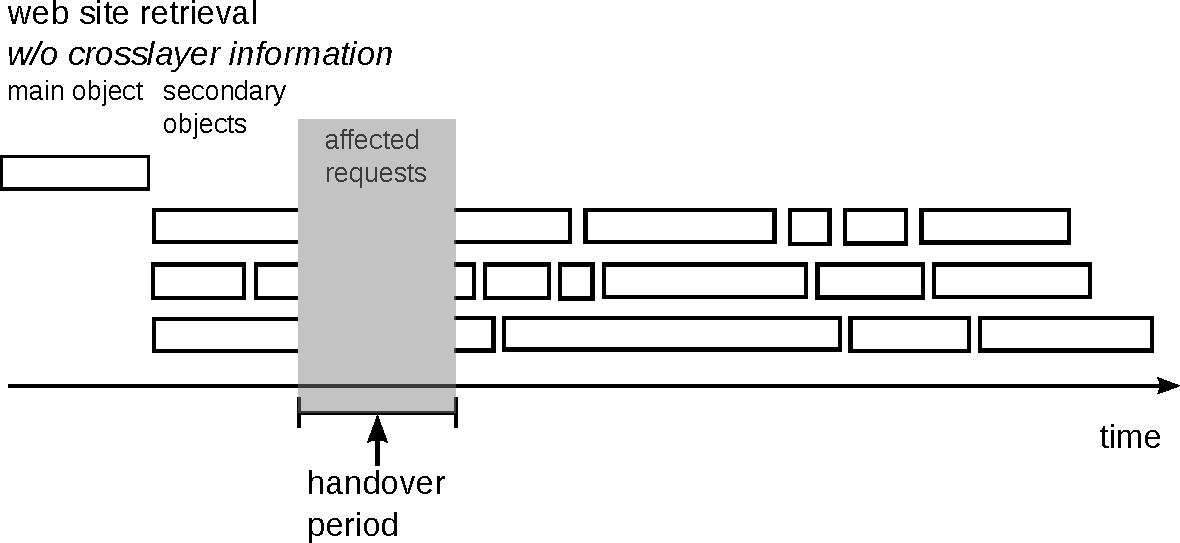
\includegraphics[width=\textwidth]{images/http-reorder-no-cl.pdf}
% 				\caption{The handover will block currently active object transmissions, page display will be delayed.}
% 				\label{c5:fig:http-reorder-no-cl}
% 	        \end{subfigure}%

% 	        \begin{subfigure}[b]{0.90\textwidth}
% 				\centering
% 				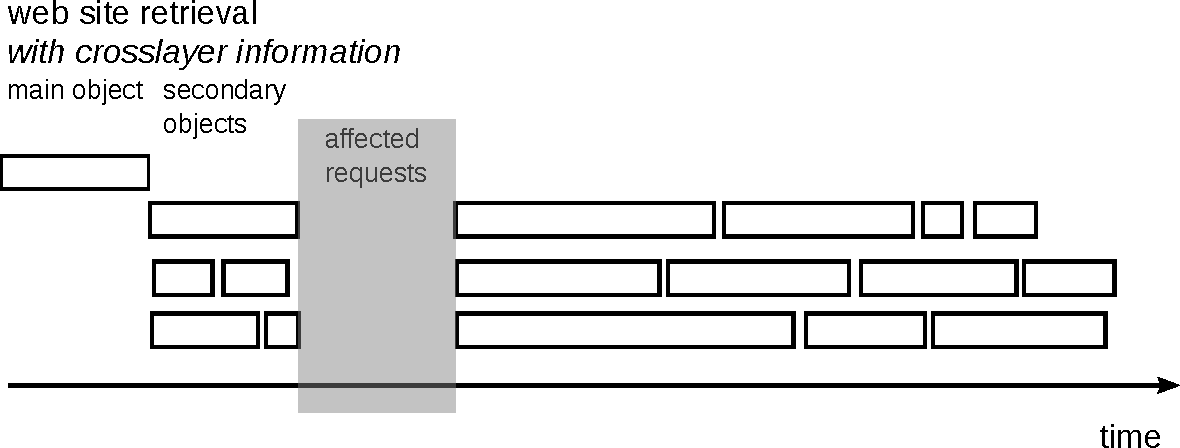
\includegraphics[width=\textwidth]{images/http-reorder-cl.pdf}
% 				\caption{The browser reorders the objects to be retrieved and avoids any transmissions during the indicated handover period.}
% 				\label{c5:fig:http-reorder-cl}
% 			   \end{subfigure}%
% 	 \caption{Mock-up of \gls{HTTP} reordering with handover awareness.}
% 	\label{c5:fig:http-reorder}
% 	\end{figure}



%Put into relation:
% \begin{itemize}
% 	\item frequency of handovers / distance/density of radio towers vs scenario traveling speed
% 	\item bit-length of streaming segments, typical transmission speed
% 	\item typical video length and number of segments
% 	\item derive number of interruptions in segments due to handovers
% 	\item estimate typical handover/mobility duration and service interruption time per event
% 	\item sum it up and compare to crosslayer information or even application layer handover decision
% \end{itemize}
%%%%%%%%%%%%%%%%%%%%%%%%%%%%%%%%%%%%%%%%%%%%%%%%%%%%%%%%%%%%%%%%%%%%%%%%%%%%%%%%



%%%%%%%%%%%%%%%
%% unused

%Characteristics of UDP packet loss: Effect of tcp traffic \cite{sawashima97characteristics}


% CoDel:
%  Head drop not tail drop
%  Queues only as shock absorbers
%  What matters is the delay within a flow
%  CoDel measures minimal packet pass through time in the local device buffer during a defined interval
%  If minimum gets too high, too much buffering is happening
%  If delay value does not once fall below a target in the interval CoDel will start dropping packets
% 	Signals congestion and hopefully reduces source rate
% 	If stays above target, progressively more packets are dropped
% 	Target: 5ms; interval: 100ms, based on simulation results
%  Can be enabled in Linux since 3.5, but many NIC drivers do not support it yet
%  Every buffer along the path influences transmission
% 	Most impact on the node before the bottleneck
% 	Cell towers, dsl/cable modems, ...

%but successful protocols develop de-facto; de jure much harder (see \gls{3G})


%protocols without retransmission feature (lost packets are not relevant and cause head-of-line blocking) but still with the all-important congestion control + TLS
%inherits new TCP features such as TFO, snap start, ...
%congestion control not through CWND but through packet pacing
%includes stream multiplexing and TLS-like crypto by default


% Multiplexing/Streams:
%  Control and Data Frames, with header compression
%  Stream interleaving/multiplexing or cancellation

%  Stream priorities (8 levels)
% 	Prefer essential resources over others (images)
% 	Prefer data with earlier deadlines? (E.g. load next few video streams immediately while already requesting more)

%  HTTP/1.1 syntax still viable as a layer on top of SPDY


% Evaluations:
% 	Average reduction in page load time: ~29\%; 27\% - 60\%
% 	Strongly dependent on connection, server environment
% 	HTTP/1.1 optimization (resources split on multiple domains) prevents SPDY multiplexing gains
%  SPDY could be more susceptible to packet loss and TCP congestion window downscaling
% 	Only one connection used compared to multiple HTTP/1.1


% IW10: better response time, still fair \cite{rfc6928}
% An argument for increasing \gls{TCP}'s initial congestion window \cite{dukkipati2010argument}
% IW3, IW10  Initial window size (IW10, ...)
%  TCP Congestion Window
% 	Maximal number of packets in flight
% –	Scaling through congestion control and avoidance algorithms
%  Initial Value
% 	1 (RFC1122, RFC2001)
% 	4000 Bytes (~ 3 packets) (RFC2414, RFC3390, ~2002)
% 	IETF proposal: IW10 
%  Rationale
% 	HTTP request for small websites using new TCP connection
% 	Transmit whole site in one RTT instead of multiple
% 	Reduces average latency
% 		Evaluation: ~10\% page load reduction on typical web pages
% 	High IW values already used by many CDNs


%Also look at ``An in-depth study of LTE: effect of network protocol and application behavior on performance'' \cite{Huang:2013:ISL:2486001.2486006}

% TCP Fast Open~\cite{cheng2014tcptfo}
%  Small server-side application adaptation required
%  Send data in the SYN and SYNACK packets
% 	Deliver it immediately to the application
% 	Only allowed for subsequent connections, requires additional security cookie (specific to client-server IP pair)
%  Saves one initial RTT
%  4\% to 41\% popular web page load time improvement

% OS-dependent receive window scaling behavior
% OS-dependent choice of packet size
% OS-dependent initial congestion window 3-10 packets
% \gls{TCP} changes (Fast Open, IW10, ...; any relationship to streaming? maybe faster)
%SACK or no SACK, CUBIC, ...

%Nagle's Algorithm~\cite{rfc896} delaying and aggregating small data packets





% TCP Early Retransmit \cite{rfc5827}
%  TCP loss recovery (not using SACK) triggers on
% 	Timeout (may be lengthy, ~RTT, min 1s)
% 	Triple duplicate ACK (fast retransmit)
% 		If CWND is small, TCP may not be able to get enough DUPACKs to trigger
% 		Reduce DUPACK threshold for these connections
% 	Less robust to segment reordering
%  Reduces average latency for narrow and lossy connections


% Proportional Rate Reduction PRR (RFC 6937 \cite{rfc6937} vs. rfc 3517)
%  TCP behavior on packet loss in the past
% 	RFC 3517: reduce CWND to half
% 		Must first ACK large portion of the data still in flight before transmitting again
% 	Linux: ``Rate halving''; Reduce CWND by 1 on every ACK until CWND/2
% 		Can still send data during recovery
%  Google IETF Proposal (Linux 3.2, January 2012): PRR
% 	Reduce timeouts by avoiding excessive window reductions
% 	Converge to cwnd chosen by congestion control by the end of recovery
% 	Can improve packet loss recovery time and average latency


%Congestion Avoidance algorithm ((New Reno~\cite{rfc6582}, Vegas~\cite{Brakmo:1994:TVN:190809.190317}, Compound~\cite{song2006compound}, BIC, CUBIC~\cite{ha2008cubic}; all w or w/o SACK)
%general basic tcp congestion control in \cite{rfc5681}, describing Reno